\chapter{Introduction}

\section{Motivation}

Environmental concerns and the challenge to improve the livability of cities are key drivers in recent urban development. Especially in cities shaped by car-centric urbanism, the car is becoming increasingly problematic due to noise and air pollution and the reduction of space due to parking requirements \cite{gossling_why_2020}. Electrifying traffic and making transportation more intelligent with cooperative transport systems is a critical aspect of reducing these negative impacts and enhancing the livability of city centers \cite{seredynski_pathways_2023}. 

In parallel, many cities are launching initiatives and pilot projects to motivate more sustainable forms of mobility, such as cycling \cite{nieuwenhuijsen_car_2016, yang_tourists_2021}. After all, expanding the distance people travel by bike leads to a direct decrease in the distance traveled by cars \cite{hatfield_effect_2016}. However, motivating more people to cycle is challenging due to two types of barriers: physical barriers and psychological barriers \cite{nieuwenhuijsen_implementing_2019}. As both types of barriers depend on each other, they can be considered a chicken-and-egg problem. Barriers that physically obstruct cyclists must first be dismantled to break down negative beliefs and attitudes toward cycling. However, this requires invasive changes to infrastructure and, consequently, citizen support. As a result, non-invasive solutions that improve the attitude towards cycling are highly desirable to accelerate the sustainable mobility transformation. 

One non-invasive possibility is making cycling smarter \cite{nikolaeva_smart_2019}. As traffic infrastructure and participants are increasingly networked, new opportunities arise for digital solutions based on the communication of traffic-related data \cite{tran_factors_2023}. Cities can provide digital solutions to cyclists that improve specific aspects of cycling as a complementary measure to other initiatives \cite{oliveira_survey_2021}. In this way, cyclists may profit from recent developments in urban data infrastructures that have so far been mainly centered on automotive applications \cite{behrendt_cycling_2019}. 

One such solution is Green Light Optimal Speed Advisory for Bikes (bike-GLOSA). This solution gives cyclists the possibility to see when the upcoming traffic light will turn green or red and provides speed advisories to ride on the green wave. The goal of such a solution is to make cycling feel more intelligent and advantageous in general, as cyclists may accelerate and reach the green phase or conserve energy by coasting. Delivered exclusively to cyclists in a city, this solution could drastically change how cycling is perceived and support the transformation to more sustainable mobility.

Hamburg has set itself this exact challenge with the PrioBike\footnote{\url{https://www.hamburg.de/bvm/priobike/}} project. One of the goals of this project is to create an app for Hamburg citizens that can be used free of charge and provides a GLOSA service for bike rides. To implement such a service, Hamburg has established an open traffic light data platform and launched a research project in collaboration with TU Dresden, which had previously developed and tested an early prototype called BikeNow \cite{frohlich_bikenow_2016, frohlich_bike_2018}. Using this prototype as an entry point, the main goal of this work is to push this idea forward, making it practical for daily use, and evaluate it on the city scale. As a central part of this process, existing solutions from the car-dominated research domain of GLOSA must be identified, and knowledge gaps for cyclist applications addressed. 

To understand the specific research gaps needed for implementing a bike-GLOSA app, we'll first examine the background research in this area. Then, we can derive more precise problems that need solving to turn the vision into reality. The remainder of our work will revolve around tackling these challenges systematically, leading to an extensive test of the system with Hamburg citizens at the end of this thesis.

\section{Background}

Services similar to Green Light Optimal Speed Advisory were proposed as early as 2006. Back then, Sanchez et al. (2006) \cite{sanchez_predicting_2006} utilized the term "Intelligent Driver Model," showing how a system could be developed that helps drivers adapt to information from an upcoming traffic light. This term was later also used in the context of model predictive control \cite{xin_predictive_2018}. In 2008, Iglesias et al. \cite{iglesias_i2v_2008} proposed a perception-enhancing "Infrastructure to Vehicle Communication Driving Assistance System" that displays a traffic light's state to the driver, increasing the distance from which the traffic light's color can be seen. The idea of a "Green Wave App" recommending speeds to the user was first introduced by Otto and Hoyer (2010) \cite{otto_operating_2010}. Tielert et al. \cite{tielert_impact_2010} introduced a "Traffic-Light-to-Vehicle-Communication" system in the same year. Then, in 2011, the term "Eco-Driving" or "Eco-Approach (and Departure)" was coined by Xia et al. (2011) \cite{xia_indirect_2011}, which would be reused over time by a few studies until today \cite{rakha_eco-driving_2011, rakha_aeris_2012, xia_field_2012, hao_eco-approach_2019, hu_lane-level_2023}. A few works in 2011 \cite{asadi_predictive_2011, raubitschek_predictive_2011} would also use the term "Predictive Cruise Control." The first work that introduced the abbreviation GLOSA was published by Katsaros et al. in 2011 \cite{katsaros_performance_2011}, which has since become established in most studies.

\begin{figure}[t]
\centering
\resizebox{\linewidth}{!}{%
\begin{tabular}{p{0.45\linewidth}p{0.55\linewidth}}
  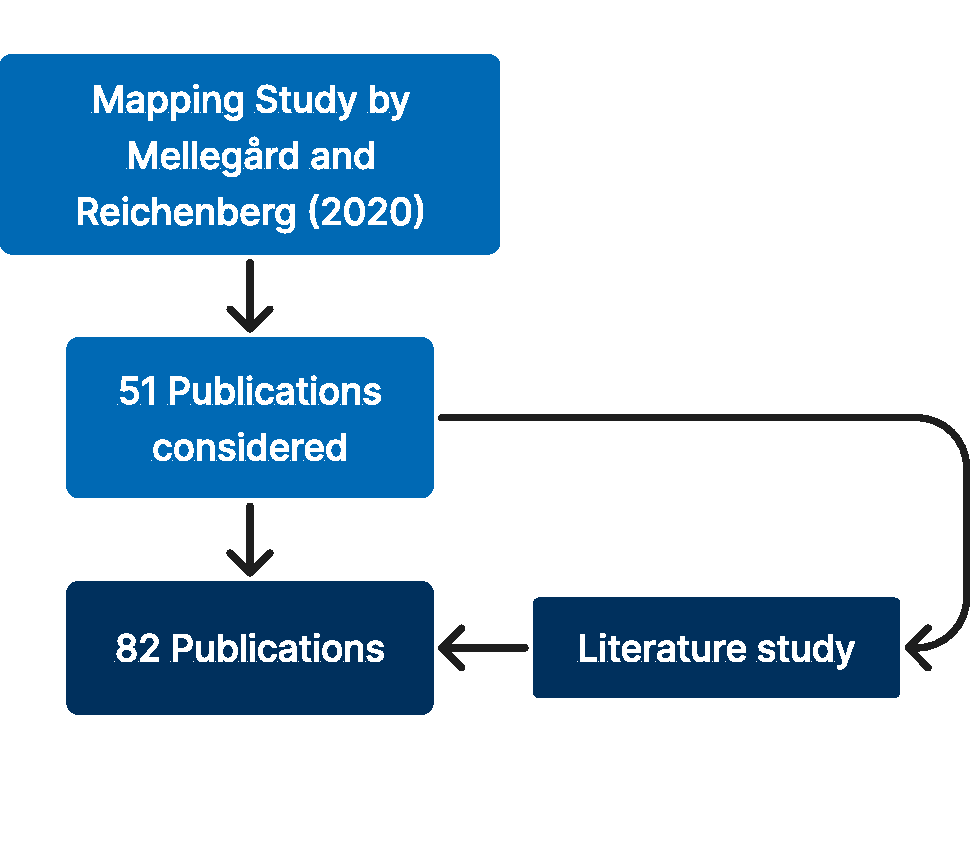
\includegraphics[width=\linewidth]{images/related-work-research-method.png} &
  \resizebox{\linewidth}{!}{%% Creator: Matplotlib, PGF backend
%%
%% To include the figure in your LaTeX document, write
%%   \input{<filename>.pgf}
%%
%% Make sure the required packages are loaded in your preamble
%%   \usepackage{pgf}
%%
%% Also ensure that all the required font packages are loaded; for instance,
%% the lmodern package is sometimes necessary when using math font.
%%   \usepackage{lmodern}
%%
%% Figures using additional raster images can only be included by \input if
%% they are in the same directory as the main LaTeX file. For loading figures
%% from other directories you can use the `import` package
%%   \usepackage{import}
%%
%% and then include the figures with
%%   \import{<path to file>}{<filename>.pgf}
%%
%% Matplotlib used the following preamble
%%   \def\mathdefault#1{#1}
%%   \everymath=\expandafter{\the\everymath\displaystyle}
%%   
%%   \makeatletter\@ifpackageloaded{underscore}{}{\usepackage[strings]{underscore}}\makeatother
%%
\begingroup%
\makeatletter%
\begin{pgfpicture}%
\pgfpathrectangle{\pgfpointorigin}{\pgfqpoint{4.490124in}{3.080266in}}%
\pgfusepath{use as bounding box, clip}%
\begin{pgfscope}%
\pgfsetbuttcap%
\pgfsetmiterjoin%
\definecolor{currentfill}{rgb}{1.000000,1.000000,1.000000}%
\pgfsetfillcolor{currentfill}%
\pgfsetlinewidth{0.000000pt}%
\definecolor{currentstroke}{rgb}{1.000000,1.000000,1.000000}%
\pgfsetstrokecolor{currentstroke}%
\pgfsetdash{}{0pt}%
\pgfpathmoveto{\pgfqpoint{0.000000in}{0.000000in}}%
\pgfpathlineto{\pgfqpoint{4.490124in}{0.000000in}}%
\pgfpathlineto{\pgfqpoint{4.490124in}{3.080266in}}%
\pgfpathlineto{\pgfqpoint{0.000000in}{3.080266in}}%
\pgfpathlineto{\pgfqpoint{0.000000in}{0.000000in}}%
\pgfpathclose%
\pgfusepath{fill}%
\end{pgfscope}%
\begin{pgfscope}%
\pgfsetbuttcap%
\pgfsetmiterjoin%
\definecolor{currentfill}{rgb}{1.000000,1.000000,1.000000}%
\pgfsetfillcolor{currentfill}%
\pgfsetlinewidth{0.000000pt}%
\definecolor{currentstroke}{rgb}{0.000000,0.000000,0.000000}%
\pgfsetstrokecolor{currentstroke}%
\pgfsetstrokeopacity{0.000000}%
\pgfsetdash{}{0pt}%
\pgfpathmoveto{\pgfqpoint{0.515124in}{0.622040in}}%
\pgfpathlineto{\pgfqpoint{4.390124in}{0.622040in}}%
\pgfpathlineto{\pgfqpoint{4.390124in}{2.932040in}}%
\pgfpathlineto{\pgfqpoint{0.515124in}{2.932040in}}%
\pgfpathlineto{\pgfqpoint{0.515124in}{0.622040in}}%
\pgfpathclose%
\pgfusepath{fill}%
\end{pgfscope}%
\begin{pgfscope}%
\pgfpathrectangle{\pgfqpoint{0.515124in}{0.622040in}}{\pgfqpoint{3.875000in}{2.310000in}}%
\pgfusepath{clip}%
\pgfsetbuttcap%
\pgfsetmiterjoin%
\definecolor{currentfill}{rgb}{0.400000,0.760784,0.647059}%
\pgfsetfillcolor{currentfill}%
\pgfsetlinewidth{0.000000pt}%
\definecolor{currentstroke}{rgb}{0.000000,0.000000,0.000000}%
\pgfsetstrokecolor{currentstroke}%
\pgfsetstrokeopacity{0.000000}%
\pgfsetdash{}{0pt}%
\pgfpathmoveto{\pgfqpoint{0.691260in}{0.622040in}}%
\pgfpathlineto{\pgfqpoint{0.840108in}{0.622040in}}%
\pgfpathlineto{\pgfqpoint{0.840108in}{0.853040in}}%
\pgfpathlineto{\pgfqpoint{0.691260in}{0.853040in}}%
\pgfpathlineto{\pgfqpoint{0.691260in}{0.622040in}}%
\pgfpathclose%
\pgfusepath{fill}%
\end{pgfscope}%
\begin{pgfscope}%
\pgfpathrectangle{\pgfqpoint{0.515124in}{0.622040in}}{\pgfqpoint{3.875000in}{2.310000in}}%
\pgfusepath{clip}%
\pgfsetbuttcap%
\pgfsetmiterjoin%
\definecolor{currentfill}{rgb}{0.400000,0.760784,0.647059}%
\pgfsetfillcolor{currentfill}%
\pgfsetlinewidth{0.000000pt}%
\definecolor{currentstroke}{rgb}{0.000000,0.000000,0.000000}%
\pgfsetstrokecolor{currentstroke}%
\pgfsetstrokeopacity{0.000000}%
\pgfsetdash{}{0pt}%
\pgfpathmoveto{\pgfqpoint{0.889724in}{0.622040in}}%
\pgfpathlineto{\pgfqpoint{1.038571in}{0.622040in}}%
\pgfpathlineto{\pgfqpoint{1.038571in}{0.622040in}}%
\pgfpathlineto{\pgfqpoint{0.889724in}{0.622040in}}%
\pgfpathlineto{\pgfqpoint{0.889724in}{0.622040in}}%
\pgfpathclose%
\pgfusepath{fill}%
\end{pgfscope}%
\begin{pgfscope}%
\pgfpathrectangle{\pgfqpoint{0.515124in}{0.622040in}}{\pgfqpoint{3.875000in}{2.310000in}}%
\pgfusepath{clip}%
\pgfsetbuttcap%
\pgfsetmiterjoin%
\definecolor{currentfill}{rgb}{0.400000,0.760784,0.647059}%
\pgfsetfillcolor{currentfill}%
\pgfsetlinewidth{0.000000pt}%
\definecolor{currentstroke}{rgb}{0.000000,0.000000,0.000000}%
\pgfsetstrokecolor{currentstroke}%
\pgfsetstrokeopacity{0.000000}%
\pgfsetdash{}{0pt}%
\pgfpathmoveto{\pgfqpoint{1.088187in}{0.622040in}}%
\pgfpathlineto{\pgfqpoint{1.237035in}{0.622040in}}%
\pgfpathlineto{\pgfqpoint{1.237035in}{0.853040in}}%
\pgfpathlineto{\pgfqpoint{1.088187in}{0.853040in}}%
\pgfpathlineto{\pgfqpoint{1.088187in}{0.622040in}}%
\pgfpathclose%
\pgfusepath{fill}%
\end{pgfscope}%
\begin{pgfscope}%
\pgfpathrectangle{\pgfqpoint{0.515124in}{0.622040in}}{\pgfqpoint{3.875000in}{2.310000in}}%
\pgfusepath{clip}%
\pgfsetbuttcap%
\pgfsetmiterjoin%
\definecolor{currentfill}{rgb}{0.400000,0.760784,0.647059}%
\pgfsetfillcolor{currentfill}%
\pgfsetlinewidth{0.000000pt}%
\definecolor{currentstroke}{rgb}{0.000000,0.000000,0.000000}%
\pgfsetstrokecolor{currentstroke}%
\pgfsetstrokeopacity{0.000000}%
\pgfsetdash{}{0pt}%
\pgfpathmoveto{\pgfqpoint{1.286651in}{0.622040in}}%
\pgfpathlineto{\pgfqpoint{1.435498in}{0.622040in}}%
\pgfpathlineto{\pgfqpoint{1.435498in}{0.622040in}}%
\pgfpathlineto{\pgfqpoint{1.286651in}{0.622040in}}%
\pgfpathlineto{\pgfqpoint{1.286651in}{0.622040in}}%
\pgfpathclose%
\pgfusepath{fill}%
\end{pgfscope}%
\begin{pgfscope}%
\pgfpathrectangle{\pgfqpoint{0.515124in}{0.622040in}}{\pgfqpoint{3.875000in}{2.310000in}}%
\pgfusepath{clip}%
\pgfsetbuttcap%
\pgfsetmiterjoin%
\definecolor{currentfill}{rgb}{0.400000,0.760784,0.647059}%
\pgfsetfillcolor{currentfill}%
\pgfsetlinewidth{0.000000pt}%
\definecolor{currentstroke}{rgb}{0.000000,0.000000,0.000000}%
\pgfsetstrokecolor{currentstroke}%
\pgfsetstrokeopacity{0.000000}%
\pgfsetdash{}{0pt}%
\pgfpathmoveto{\pgfqpoint{1.485114in}{0.622040in}}%
\pgfpathlineto{\pgfqpoint{1.633962in}{0.622040in}}%
\pgfpathlineto{\pgfqpoint{1.633962in}{0.853040in}}%
\pgfpathlineto{\pgfqpoint{1.485114in}{0.853040in}}%
\pgfpathlineto{\pgfqpoint{1.485114in}{0.622040in}}%
\pgfpathclose%
\pgfusepath{fill}%
\end{pgfscope}%
\begin{pgfscope}%
\pgfpathrectangle{\pgfqpoint{0.515124in}{0.622040in}}{\pgfqpoint{3.875000in}{2.310000in}}%
\pgfusepath{clip}%
\pgfsetbuttcap%
\pgfsetmiterjoin%
\definecolor{currentfill}{rgb}{0.400000,0.760784,0.647059}%
\pgfsetfillcolor{currentfill}%
\pgfsetlinewidth{0.000000pt}%
\definecolor{currentstroke}{rgb}{0.000000,0.000000,0.000000}%
\pgfsetstrokecolor{currentstroke}%
\pgfsetstrokeopacity{0.000000}%
\pgfsetdash{}{0pt}%
\pgfpathmoveto{\pgfqpoint{1.683578in}{0.622040in}}%
\pgfpathlineto{\pgfqpoint{1.832425in}{0.622040in}}%
\pgfpathlineto{\pgfqpoint{1.832425in}{2.239040in}}%
\pgfpathlineto{\pgfqpoint{1.683578in}{2.239040in}}%
\pgfpathlineto{\pgfqpoint{1.683578in}{0.622040in}}%
\pgfpathclose%
\pgfusepath{fill}%
\end{pgfscope}%
\begin{pgfscope}%
\pgfpathrectangle{\pgfqpoint{0.515124in}{0.622040in}}{\pgfqpoint{3.875000in}{2.310000in}}%
\pgfusepath{clip}%
\pgfsetbuttcap%
\pgfsetmiterjoin%
\definecolor{currentfill}{rgb}{0.400000,0.760784,0.647059}%
\pgfsetfillcolor{currentfill}%
\pgfsetlinewidth{0.000000pt}%
\definecolor{currentstroke}{rgb}{0.000000,0.000000,0.000000}%
\pgfsetstrokecolor{currentstroke}%
\pgfsetstrokeopacity{0.000000}%
\pgfsetdash{}{0pt}%
\pgfpathmoveto{\pgfqpoint{1.882041in}{0.622040in}}%
\pgfpathlineto{\pgfqpoint{2.030889in}{0.622040in}}%
\pgfpathlineto{\pgfqpoint{2.030889in}{2.008040in}}%
\pgfpathlineto{\pgfqpoint{1.882041in}{2.008040in}}%
\pgfpathlineto{\pgfqpoint{1.882041in}{0.622040in}}%
\pgfpathclose%
\pgfusepath{fill}%
\end{pgfscope}%
\begin{pgfscope}%
\pgfpathrectangle{\pgfqpoint{0.515124in}{0.622040in}}{\pgfqpoint{3.875000in}{2.310000in}}%
\pgfusepath{clip}%
\pgfsetbuttcap%
\pgfsetmiterjoin%
\definecolor{currentfill}{rgb}{0.400000,0.760784,0.647059}%
\pgfsetfillcolor{currentfill}%
\pgfsetlinewidth{0.000000pt}%
\definecolor{currentstroke}{rgb}{0.000000,0.000000,0.000000}%
\pgfsetstrokecolor{currentstroke}%
\pgfsetstrokeopacity{0.000000}%
\pgfsetdash{}{0pt}%
\pgfpathmoveto{\pgfqpoint{2.080505in}{0.622040in}}%
\pgfpathlineto{\pgfqpoint{2.229352in}{0.622040in}}%
\pgfpathlineto{\pgfqpoint{2.229352in}{2.239040in}}%
\pgfpathlineto{\pgfqpoint{2.080505in}{2.239040in}}%
\pgfpathlineto{\pgfqpoint{2.080505in}{0.622040in}}%
\pgfpathclose%
\pgfusepath{fill}%
\end{pgfscope}%
\begin{pgfscope}%
\pgfpathrectangle{\pgfqpoint{0.515124in}{0.622040in}}{\pgfqpoint{3.875000in}{2.310000in}}%
\pgfusepath{clip}%
\pgfsetbuttcap%
\pgfsetmiterjoin%
\definecolor{currentfill}{rgb}{0.400000,0.760784,0.647059}%
\pgfsetfillcolor{currentfill}%
\pgfsetlinewidth{0.000000pt}%
\definecolor{currentstroke}{rgb}{0.000000,0.000000,0.000000}%
\pgfsetstrokecolor{currentstroke}%
\pgfsetstrokeopacity{0.000000}%
\pgfsetdash{}{0pt}%
\pgfpathmoveto{\pgfqpoint{2.278968in}{0.622040in}}%
\pgfpathlineto{\pgfqpoint{2.427816in}{0.622040in}}%
\pgfpathlineto{\pgfqpoint{2.427816in}{1.777040in}}%
\pgfpathlineto{\pgfqpoint{2.278968in}{1.777040in}}%
\pgfpathlineto{\pgfqpoint{2.278968in}{0.622040in}}%
\pgfpathclose%
\pgfusepath{fill}%
\end{pgfscope}%
\begin{pgfscope}%
\pgfpathrectangle{\pgfqpoint{0.515124in}{0.622040in}}{\pgfqpoint{3.875000in}{2.310000in}}%
\pgfusepath{clip}%
\pgfsetbuttcap%
\pgfsetmiterjoin%
\definecolor{currentfill}{rgb}{0.400000,0.760784,0.647059}%
\pgfsetfillcolor{currentfill}%
\pgfsetlinewidth{0.000000pt}%
\definecolor{currentstroke}{rgb}{0.000000,0.000000,0.000000}%
\pgfsetstrokecolor{currentstroke}%
\pgfsetstrokeopacity{0.000000}%
\pgfsetdash{}{0pt}%
\pgfpathmoveto{\pgfqpoint{2.477432in}{0.622040in}}%
\pgfpathlineto{\pgfqpoint{2.626279in}{0.622040in}}%
\pgfpathlineto{\pgfqpoint{2.626279in}{1.084040in}}%
\pgfpathlineto{\pgfqpoint{2.477432in}{1.084040in}}%
\pgfpathlineto{\pgfqpoint{2.477432in}{0.622040in}}%
\pgfpathclose%
\pgfusepath{fill}%
\end{pgfscope}%
\begin{pgfscope}%
\pgfpathrectangle{\pgfqpoint{0.515124in}{0.622040in}}{\pgfqpoint{3.875000in}{2.310000in}}%
\pgfusepath{clip}%
\pgfsetbuttcap%
\pgfsetmiterjoin%
\definecolor{currentfill}{rgb}{0.400000,0.760784,0.647059}%
\pgfsetfillcolor{currentfill}%
\pgfsetlinewidth{0.000000pt}%
\definecolor{currentstroke}{rgb}{0.000000,0.000000,0.000000}%
\pgfsetstrokecolor{currentstroke}%
\pgfsetstrokeopacity{0.000000}%
\pgfsetdash{}{0pt}%
\pgfpathmoveto{\pgfqpoint{2.675895in}{0.622040in}}%
\pgfpathlineto{\pgfqpoint{2.824743in}{0.622040in}}%
\pgfpathlineto{\pgfqpoint{2.824743in}{1.777040in}}%
\pgfpathlineto{\pgfqpoint{2.675895in}{1.777040in}}%
\pgfpathlineto{\pgfqpoint{2.675895in}{0.622040in}}%
\pgfpathclose%
\pgfusepath{fill}%
\end{pgfscope}%
\begin{pgfscope}%
\pgfpathrectangle{\pgfqpoint{0.515124in}{0.622040in}}{\pgfqpoint{3.875000in}{2.310000in}}%
\pgfusepath{clip}%
\pgfsetbuttcap%
\pgfsetmiterjoin%
\definecolor{currentfill}{rgb}{0.400000,0.760784,0.647059}%
\pgfsetfillcolor{currentfill}%
\pgfsetlinewidth{0.000000pt}%
\definecolor{currentstroke}{rgb}{0.000000,0.000000,0.000000}%
\pgfsetstrokecolor{currentstroke}%
\pgfsetstrokeopacity{0.000000}%
\pgfsetdash{}{0pt}%
\pgfpathmoveto{\pgfqpoint{2.874359in}{0.622040in}}%
\pgfpathlineto{\pgfqpoint{3.023206in}{0.622040in}}%
\pgfpathlineto{\pgfqpoint{3.023206in}{1.084040in}}%
\pgfpathlineto{\pgfqpoint{2.874359in}{1.084040in}}%
\pgfpathlineto{\pgfqpoint{2.874359in}{0.622040in}}%
\pgfpathclose%
\pgfusepath{fill}%
\end{pgfscope}%
\begin{pgfscope}%
\pgfpathrectangle{\pgfqpoint{0.515124in}{0.622040in}}{\pgfqpoint{3.875000in}{2.310000in}}%
\pgfusepath{clip}%
\pgfsetbuttcap%
\pgfsetmiterjoin%
\definecolor{currentfill}{rgb}{0.400000,0.760784,0.647059}%
\pgfsetfillcolor{currentfill}%
\pgfsetlinewidth{0.000000pt}%
\definecolor{currentstroke}{rgb}{0.000000,0.000000,0.000000}%
\pgfsetstrokecolor{currentstroke}%
\pgfsetstrokeopacity{0.000000}%
\pgfsetdash{}{0pt}%
\pgfpathmoveto{\pgfqpoint{3.072822in}{0.622040in}}%
\pgfpathlineto{\pgfqpoint{3.221670in}{0.622040in}}%
\pgfpathlineto{\pgfqpoint{3.221670in}{2.239040in}}%
\pgfpathlineto{\pgfqpoint{3.072822in}{2.239040in}}%
\pgfpathlineto{\pgfqpoint{3.072822in}{0.622040in}}%
\pgfpathclose%
\pgfusepath{fill}%
\end{pgfscope}%
\begin{pgfscope}%
\pgfpathrectangle{\pgfqpoint{0.515124in}{0.622040in}}{\pgfqpoint{3.875000in}{2.310000in}}%
\pgfusepath{clip}%
\pgfsetbuttcap%
\pgfsetmiterjoin%
\definecolor{currentfill}{rgb}{0.400000,0.760784,0.647059}%
\pgfsetfillcolor{currentfill}%
\pgfsetlinewidth{0.000000pt}%
\definecolor{currentstroke}{rgb}{0.000000,0.000000,0.000000}%
\pgfsetstrokecolor{currentstroke}%
\pgfsetstrokeopacity{0.000000}%
\pgfsetdash{}{0pt}%
\pgfpathmoveto{\pgfqpoint{3.271286in}{0.622040in}}%
\pgfpathlineto{\pgfqpoint{3.420133in}{0.622040in}}%
\pgfpathlineto{\pgfqpoint{3.420133in}{1.084040in}}%
\pgfpathlineto{\pgfqpoint{3.271286in}{1.084040in}}%
\pgfpathlineto{\pgfqpoint{3.271286in}{0.622040in}}%
\pgfpathclose%
\pgfusepath{fill}%
\end{pgfscope}%
\begin{pgfscope}%
\pgfpathrectangle{\pgfqpoint{0.515124in}{0.622040in}}{\pgfqpoint{3.875000in}{2.310000in}}%
\pgfusepath{clip}%
\pgfsetbuttcap%
\pgfsetmiterjoin%
\definecolor{currentfill}{rgb}{0.400000,0.760784,0.647059}%
\pgfsetfillcolor{currentfill}%
\pgfsetlinewidth{0.000000pt}%
\definecolor{currentstroke}{rgb}{0.000000,0.000000,0.000000}%
\pgfsetstrokecolor{currentstroke}%
\pgfsetstrokeopacity{0.000000}%
\pgfsetdash{}{0pt}%
\pgfpathmoveto{\pgfqpoint{3.469749in}{0.622040in}}%
\pgfpathlineto{\pgfqpoint{3.618597in}{0.622040in}}%
\pgfpathlineto{\pgfqpoint{3.618597in}{0.622040in}}%
\pgfpathlineto{\pgfqpoint{3.469749in}{0.622040in}}%
\pgfpathlineto{\pgfqpoint{3.469749in}{0.622040in}}%
\pgfpathclose%
\pgfusepath{fill}%
\end{pgfscope}%
\begin{pgfscope}%
\pgfpathrectangle{\pgfqpoint{0.515124in}{0.622040in}}{\pgfqpoint{3.875000in}{2.310000in}}%
\pgfusepath{clip}%
\pgfsetbuttcap%
\pgfsetmiterjoin%
\definecolor{currentfill}{rgb}{0.400000,0.760784,0.647059}%
\pgfsetfillcolor{currentfill}%
\pgfsetlinewidth{0.000000pt}%
\definecolor{currentstroke}{rgb}{0.000000,0.000000,0.000000}%
\pgfsetstrokecolor{currentstroke}%
\pgfsetstrokeopacity{0.000000}%
\pgfsetdash{}{0pt}%
\pgfpathmoveto{\pgfqpoint{3.668213in}{0.622040in}}%
\pgfpathlineto{\pgfqpoint{3.817060in}{0.622040in}}%
\pgfpathlineto{\pgfqpoint{3.817060in}{0.622040in}}%
\pgfpathlineto{\pgfqpoint{3.668213in}{0.622040in}}%
\pgfpathlineto{\pgfqpoint{3.668213in}{0.622040in}}%
\pgfpathclose%
\pgfusepath{fill}%
\end{pgfscope}%
\begin{pgfscope}%
\pgfpathrectangle{\pgfqpoint{0.515124in}{0.622040in}}{\pgfqpoint{3.875000in}{2.310000in}}%
\pgfusepath{clip}%
\pgfsetbuttcap%
\pgfsetmiterjoin%
\definecolor{currentfill}{rgb}{0.400000,0.760784,0.647059}%
\pgfsetfillcolor{currentfill}%
\pgfsetlinewidth{0.000000pt}%
\definecolor{currentstroke}{rgb}{0.000000,0.000000,0.000000}%
\pgfsetstrokecolor{currentstroke}%
\pgfsetstrokeopacity{0.000000}%
\pgfsetdash{}{0pt}%
\pgfpathmoveto{\pgfqpoint{3.866676in}{0.622040in}}%
\pgfpathlineto{\pgfqpoint{4.015524in}{0.622040in}}%
\pgfpathlineto{\pgfqpoint{4.015524in}{0.622040in}}%
\pgfpathlineto{\pgfqpoint{3.866676in}{0.622040in}}%
\pgfpathlineto{\pgfqpoint{3.866676in}{0.622040in}}%
\pgfpathclose%
\pgfusepath{fill}%
\end{pgfscope}%
\begin{pgfscope}%
\pgfpathrectangle{\pgfqpoint{0.515124in}{0.622040in}}{\pgfqpoint{3.875000in}{2.310000in}}%
\pgfusepath{clip}%
\pgfsetbuttcap%
\pgfsetmiterjoin%
\definecolor{currentfill}{rgb}{0.400000,0.760784,0.647059}%
\pgfsetfillcolor{currentfill}%
\pgfsetlinewidth{0.000000pt}%
\definecolor{currentstroke}{rgb}{0.000000,0.000000,0.000000}%
\pgfsetstrokecolor{currentstroke}%
\pgfsetstrokeopacity{0.000000}%
\pgfsetdash{}{0pt}%
\pgfpathmoveto{\pgfqpoint{4.065140in}{0.622040in}}%
\pgfpathlineto{\pgfqpoint{4.213987in}{0.622040in}}%
\pgfpathlineto{\pgfqpoint{4.213987in}{0.622040in}}%
\pgfpathlineto{\pgfqpoint{4.065140in}{0.622040in}}%
\pgfpathlineto{\pgfqpoint{4.065140in}{0.622040in}}%
\pgfpathclose%
\pgfusepath{fill}%
\end{pgfscope}%
\begin{pgfscope}%
\pgfpathrectangle{\pgfqpoint{0.515124in}{0.622040in}}{\pgfqpoint{3.875000in}{2.310000in}}%
\pgfusepath{clip}%
\pgfsetbuttcap%
\pgfsetmiterjoin%
\definecolor{currentfill}{rgb}{0.988235,0.552941,0.384314}%
\pgfsetfillcolor{currentfill}%
\pgfsetlinewidth{0.000000pt}%
\definecolor{currentstroke}{rgb}{0.000000,0.000000,0.000000}%
\pgfsetstrokecolor{currentstroke}%
\pgfsetstrokeopacity{0.000000}%
\pgfsetdash{}{0pt}%
\pgfpathmoveto{\pgfqpoint{0.691260in}{0.853040in}}%
\pgfpathlineto{\pgfqpoint{0.840108in}{0.853040in}}%
\pgfpathlineto{\pgfqpoint{0.840108in}{0.853040in}}%
\pgfpathlineto{\pgfqpoint{0.691260in}{0.853040in}}%
\pgfpathlineto{\pgfqpoint{0.691260in}{0.853040in}}%
\pgfpathclose%
\pgfusepath{fill}%
\end{pgfscope}%
\begin{pgfscope}%
\pgfpathrectangle{\pgfqpoint{0.515124in}{0.622040in}}{\pgfqpoint{3.875000in}{2.310000in}}%
\pgfusepath{clip}%
\pgfsetbuttcap%
\pgfsetmiterjoin%
\definecolor{currentfill}{rgb}{0.988235,0.552941,0.384314}%
\pgfsetfillcolor{currentfill}%
\pgfsetlinewidth{0.000000pt}%
\definecolor{currentstroke}{rgb}{0.000000,0.000000,0.000000}%
\pgfsetstrokecolor{currentstroke}%
\pgfsetstrokeopacity{0.000000}%
\pgfsetdash{}{0pt}%
\pgfpathmoveto{\pgfqpoint{0.889724in}{0.622040in}}%
\pgfpathlineto{\pgfqpoint{1.038571in}{0.622040in}}%
\pgfpathlineto{\pgfqpoint{1.038571in}{0.622040in}}%
\pgfpathlineto{\pgfqpoint{0.889724in}{0.622040in}}%
\pgfpathlineto{\pgfqpoint{0.889724in}{0.622040in}}%
\pgfpathclose%
\pgfusepath{fill}%
\end{pgfscope}%
\begin{pgfscope}%
\pgfpathrectangle{\pgfqpoint{0.515124in}{0.622040in}}{\pgfqpoint{3.875000in}{2.310000in}}%
\pgfusepath{clip}%
\pgfsetbuttcap%
\pgfsetmiterjoin%
\definecolor{currentfill}{rgb}{0.988235,0.552941,0.384314}%
\pgfsetfillcolor{currentfill}%
\pgfsetlinewidth{0.000000pt}%
\definecolor{currentstroke}{rgb}{0.000000,0.000000,0.000000}%
\pgfsetstrokecolor{currentstroke}%
\pgfsetstrokeopacity{0.000000}%
\pgfsetdash{}{0pt}%
\pgfpathmoveto{\pgfqpoint{1.088187in}{0.853040in}}%
\pgfpathlineto{\pgfqpoint{1.237035in}{0.853040in}}%
\pgfpathlineto{\pgfqpoint{1.237035in}{0.853040in}}%
\pgfpathlineto{\pgfqpoint{1.088187in}{0.853040in}}%
\pgfpathlineto{\pgfqpoint{1.088187in}{0.853040in}}%
\pgfpathclose%
\pgfusepath{fill}%
\end{pgfscope}%
\begin{pgfscope}%
\pgfpathrectangle{\pgfqpoint{0.515124in}{0.622040in}}{\pgfqpoint{3.875000in}{2.310000in}}%
\pgfusepath{clip}%
\pgfsetbuttcap%
\pgfsetmiterjoin%
\definecolor{currentfill}{rgb}{0.988235,0.552941,0.384314}%
\pgfsetfillcolor{currentfill}%
\pgfsetlinewidth{0.000000pt}%
\definecolor{currentstroke}{rgb}{0.000000,0.000000,0.000000}%
\pgfsetstrokecolor{currentstroke}%
\pgfsetstrokeopacity{0.000000}%
\pgfsetdash{}{0pt}%
\pgfpathmoveto{\pgfqpoint{1.286651in}{0.622040in}}%
\pgfpathlineto{\pgfqpoint{1.435498in}{0.622040in}}%
\pgfpathlineto{\pgfqpoint{1.435498in}{0.622040in}}%
\pgfpathlineto{\pgfqpoint{1.286651in}{0.622040in}}%
\pgfpathlineto{\pgfqpoint{1.286651in}{0.622040in}}%
\pgfpathclose%
\pgfusepath{fill}%
\end{pgfscope}%
\begin{pgfscope}%
\pgfpathrectangle{\pgfqpoint{0.515124in}{0.622040in}}{\pgfqpoint{3.875000in}{2.310000in}}%
\pgfusepath{clip}%
\pgfsetbuttcap%
\pgfsetmiterjoin%
\definecolor{currentfill}{rgb}{0.988235,0.552941,0.384314}%
\pgfsetfillcolor{currentfill}%
\pgfsetlinewidth{0.000000pt}%
\definecolor{currentstroke}{rgb}{0.000000,0.000000,0.000000}%
\pgfsetstrokecolor{currentstroke}%
\pgfsetstrokeopacity{0.000000}%
\pgfsetdash{}{0pt}%
\pgfpathmoveto{\pgfqpoint{1.485114in}{0.853040in}}%
\pgfpathlineto{\pgfqpoint{1.633962in}{0.853040in}}%
\pgfpathlineto{\pgfqpoint{1.633962in}{1.084040in}}%
\pgfpathlineto{\pgfqpoint{1.485114in}{1.084040in}}%
\pgfpathlineto{\pgfqpoint{1.485114in}{0.853040in}}%
\pgfpathclose%
\pgfusepath{fill}%
\end{pgfscope}%
\begin{pgfscope}%
\pgfpathrectangle{\pgfqpoint{0.515124in}{0.622040in}}{\pgfqpoint{3.875000in}{2.310000in}}%
\pgfusepath{clip}%
\pgfsetbuttcap%
\pgfsetmiterjoin%
\definecolor{currentfill}{rgb}{0.988235,0.552941,0.384314}%
\pgfsetfillcolor{currentfill}%
\pgfsetlinewidth{0.000000pt}%
\definecolor{currentstroke}{rgb}{0.000000,0.000000,0.000000}%
\pgfsetstrokecolor{currentstroke}%
\pgfsetstrokeopacity{0.000000}%
\pgfsetdash{}{0pt}%
\pgfpathmoveto{\pgfqpoint{1.683578in}{2.239040in}}%
\pgfpathlineto{\pgfqpoint{1.832425in}{2.239040in}}%
\pgfpathlineto{\pgfqpoint{1.832425in}{2.239040in}}%
\pgfpathlineto{\pgfqpoint{1.683578in}{2.239040in}}%
\pgfpathlineto{\pgfqpoint{1.683578in}{2.239040in}}%
\pgfpathclose%
\pgfusepath{fill}%
\end{pgfscope}%
\begin{pgfscope}%
\pgfpathrectangle{\pgfqpoint{0.515124in}{0.622040in}}{\pgfqpoint{3.875000in}{2.310000in}}%
\pgfusepath{clip}%
\pgfsetbuttcap%
\pgfsetmiterjoin%
\definecolor{currentfill}{rgb}{0.988235,0.552941,0.384314}%
\pgfsetfillcolor{currentfill}%
\pgfsetlinewidth{0.000000pt}%
\definecolor{currentstroke}{rgb}{0.000000,0.000000,0.000000}%
\pgfsetstrokecolor{currentstroke}%
\pgfsetstrokeopacity{0.000000}%
\pgfsetdash{}{0pt}%
\pgfpathmoveto{\pgfqpoint{1.882041in}{2.008040in}}%
\pgfpathlineto{\pgfqpoint{2.030889in}{2.008040in}}%
\pgfpathlineto{\pgfqpoint{2.030889in}{2.239040in}}%
\pgfpathlineto{\pgfqpoint{1.882041in}{2.239040in}}%
\pgfpathlineto{\pgfqpoint{1.882041in}{2.008040in}}%
\pgfpathclose%
\pgfusepath{fill}%
\end{pgfscope}%
\begin{pgfscope}%
\pgfpathrectangle{\pgfqpoint{0.515124in}{0.622040in}}{\pgfqpoint{3.875000in}{2.310000in}}%
\pgfusepath{clip}%
\pgfsetbuttcap%
\pgfsetmiterjoin%
\definecolor{currentfill}{rgb}{0.988235,0.552941,0.384314}%
\pgfsetfillcolor{currentfill}%
\pgfsetlinewidth{0.000000pt}%
\definecolor{currentstroke}{rgb}{0.000000,0.000000,0.000000}%
\pgfsetstrokecolor{currentstroke}%
\pgfsetstrokeopacity{0.000000}%
\pgfsetdash{}{0pt}%
\pgfpathmoveto{\pgfqpoint{2.080505in}{2.239040in}}%
\pgfpathlineto{\pgfqpoint{2.229352in}{2.239040in}}%
\pgfpathlineto{\pgfqpoint{2.229352in}{2.239040in}}%
\pgfpathlineto{\pgfqpoint{2.080505in}{2.239040in}}%
\pgfpathlineto{\pgfqpoint{2.080505in}{2.239040in}}%
\pgfpathclose%
\pgfusepath{fill}%
\end{pgfscope}%
\begin{pgfscope}%
\pgfpathrectangle{\pgfqpoint{0.515124in}{0.622040in}}{\pgfqpoint{3.875000in}{2.310000in}}%
\pgfusepath{clip}%
\pgfsetbuttcap%
\pgfsetmiterjoin%
\definecolor{currentfill}{rgb}{0.988235,0.552941,0.384314}%
\pgfsetfillcolor{currentfill}%
\pgfsetlinewidth{0.000000pt}%
\definecolor{currentstroke}{rgb}{0.000000,0.000000,0.000000}%
\pgfsetstrokecolor{currentstroke}%
\pgfsetstrokeopacity{0.000000}%
\pgfsetdash{}{0pt}%
\pgfpathmoveto{\pgfqpoint{2.278968in}{1.777040in}}%
\pgfpathlineto{\pgfqpoint{2.427816in}{1.777040in}}%
\pgfpathlineto{\pgfqpoint{2.427816in}{1.777040in}}%
\pgfpathlineto{\pgfqpoint{2.278968in}{1.777040in}}%
\pgfpathlineto{\pgfqpoint{2.278968in}{1.777040in}}%
\pgfpathclose%
\pgfusepath{fill}%
\end{pgfscope}%
\begin{pgfscope}%
\pgfpathrectangle{\pgfqpoint{0.515124in}{0.622040in}}{\pgfqpoint{3.875000in}{2.310000in}}%
\pgfusepath{clip}%
\pgfsetbuttcap%
\pgfsetmiterjoin%
\definecolor{currentfill}{rgb}{0.988235,0.552941,0.384314}%
\pgfsetfillcolor{currentfill}%
\pgfsetlinewidth{0.000000pt}%
\definecolor{currentstroke}{rgb}{0.000000,0.000000,0.000000}%
\pgfsetstrokecolor{currentstroke}%
\pgfsetstrokeopacity{0.000000}%
\pgfsetdash{}{0pt}%
\pgfpathmoveto{\pgfqpoint{2.477432in}{1.084040in}}%
\pgfpathlineto{\pgfqpoint{2.626279in}{1.084040in}}%
\pgfpathlineto{\pgfqpoint{2.626279in}{1.315040in}}%
\pgfpathlineto{\pgfqpoint{2.477432in}{1.315040in}}%
\pgfpathlineto{\pgfqpoint{2.477432in}{1.084040in}}%
\pgfpathclose%
\pgfusepath{fill}%
\end{pgfscope}%
\begin{pgfscope}%
\pgfpathrectangle{\pgfqpoint{0.515124in}{0.622040in}}{\pgfqpoint{3.875000in}{2.310000in}}%
\pgfusepath{clip}%
\pgfsetbuttcap%
\pgfsetmiterjoin%
\definecolor{currentfill}{rgb}{0.988235,0.552941,0.384314}%
\pgfsetfillcolor{currentfill}%
\pgfsetlinewidth{0.000000pt}%
\definecolor{currentstroke}{rgb}{0.000000,0.000000,0.000000}%
\pgfsetstrokecolor{currentstroke}%
\pgfsetstrokeopacity{0.000000}%
\pgfsetdash{}{0pt}%
\pgfpathmoveto{\pgfqpoint{2.675895in}{1.777040in}}%
\pgfpathlineto{\pgfqpoint{2.824743in}{1.777040in}}%
\pgfpathlineto{\pgfqpoint{2.824743in}{1.777040in}}%
\pgfpathlineto{\pgfqpoint{2.675895in}{1.777040in}}%
\pgfpathlineto{\pgfqpoint{2.675895in}{1.777040in}}%
\pgfpathclose%
\pgfusepath{fill}%
\end{pgfscope}%
\begin{pgfscope}%
\pgfpathrectangle{\pgfqpoint{0.515124in}{0.622040in}}{\pgfqpoint{3.875000in}{2.310000in}}%
\pgfusepath{clip}%
\pgfsetbuttcap%
\pgfsetmiterjoin%
\definecolor{currentfill}{rgb}{0.988235,0.552941,0.384314}%
\pgfsetfillcolor{currentfill}%
\pgfsetlinewidth{0.000000pt}%
\definecolor{currentstroke}{rgb}{0.000000,0.000000,0.000000}%
\pgfsetstrokecolor{currentstroke}%
\pgfsetstrokeopacity{0.000000}%
\pgfsetdash{}{0pt}%
\pgfpathmoveto{\pgfqpoint{2.874359in}{1.084040in}}%
\pgfpathlineto{\pgfqpoint{3.023206in}{1.084040in}}%
\pgfpathlineto{\pgfqpoint{3.023206in}{1.546040in}}%
\pgfpathlineto{\pgfqpoint{2.874359in}{1.546040in}}%
\pgfpathlineto{\pgfqpoint{2.874359in}{1.084040in}}%
\pgfpathclose%
\pgfusepath{fill}%
\end{pgfscope}%
\begin{pgfscope}%
\pgfpathrectangle{\pgfqpoint{0.515124in}{0.622040in}}{\pgfqpoint{3.875000in}{2.310000in}}%
\pgfusepath{clip}%
\pgfsetbuttcap%
\pgfsetmiterjoin%
\definecolor{currentfill}{rgb}{0.988235,0.552941,0.384314}%
\pgfsetfillcolor{currentfill}%
\pgfsetlinewidth{0.000000pt}%
\definecolor{currentstroke}{rgb}{0.000000,0.000000,0.000000}%
\pgfsetstrokecolor{currentstroke}%
\pgfsetstrokeopacity{0.000000}%
\pgfsetdash{}{0pt}%
\pgfpathmoveto{\pgfqpoint{3.072822in}{2.239040in}}%
\pgfpathlineto{\pgfqpoint{3.221670in}{2.239040in}}%
\pgfpathlineto{\pgfqpoint{3.221670in}{2.470040in}}%
\pgfpathlineto{\pgfqpoint{3.072822in}{2.470040in}}%
\pgfpathlineto{\pgfqpoint{3.072822in}{2.239040in}}%
\pgfpathclose%
\pgfusepath{fill}%
\end{pgfscope}%
\begin{pgfscope}%
\pgfpathrectangle{\pgfqpoint{0.515124in}{0.622040in}}{\pgfqpoint{3.875000in}{2.310000in}}%
\pgfusepath{clip}%
\pgfsetbuttcap%
\pgfsetmiterjoin%
\definecolor{currentfill}{rgb}{0.988235,0.552941,0.384314}%
\pgfsetfillcolor{currentfill}%
\pgfsetlinewidth{0.000000pt}%
\definecolor{currentstroke}{rgb}{0.000000,0.000000,0.000000}%
\pgfsetstrokecolor{currentstroke}%
\pgfsetstrokeopacity{0.000000}%
\pgfsetdash{}{0pt}%
\pgfpathmoveto{\pgfqpoint{3.271286in}{1.084040in}}%
\pgfpathlineto{\pgfqpoint{3.420133in}{1.084040in}}%
\pgfpathlineto{\pgfqpoint{3.420133in}{1.777040in}}%
\pgfpathlineto{\pgfqpoint{3.271286in}{1.777040in}}%
\pgfpathlineto{\pgfqpoint{3.271286in}{1.084040in}}%
\pgfpathclose%
\pgfusepath{fill}%
\end{pgfscope}%
\begin{pgfscope}%
\pgfpathrectangle{\pgfqpoint{0.515124in}{0.622040in}}{\pgfqpoint{3.875000in}{2.310000in}}%
\pgfusepath{clip}%
\pgfsetbuttcap%
\pgfsetmiterjoin%
\definecolor{currentfill}{rgb}{0.988235,0.552941,0.384314}%
\pgfsetfillcolor{currentfill}%
\pgfsetlinewidth{0.000000pt}%
\definecolor{currentstroke}{rgb}{0.000000,0.000000,0.000000}%
\pgfsetstrokecolor{currentstroke}%
\pgfsetstrokeopacity{0.000000}%
\pgfsetdash{}{0pt}%
\pgfpathmoveto{\pgfqpoint{3.469749in}{0.622040in}}%
\pgfpathlineto{\pgfqpoint{3.618597in}{0.622040in}}%
\pgfpathlineto{\pgfqpoint{3.618597in}{1.777040in}}%
\pgfpathlineto{\pgfqpoint{3.469749in}{1.777040in}}%
\pgfpathlineto{\pgfqpoint{3.469749in}{0.622040in}}%
\pgfpathclose%
\pgfusepath{fill}%
\end{pgfscope}%
\begin{pgfscope}%
\pgfpathrectangle{\pgfqpoint{0.515124in}{0.622040in}}{\pgfqpoint{3.875000in}{2.310000in}}%
\pgfusepath{clip}%
\pgfsetbuttcap%
\pgfsetmiterjoin%
\definecolor{currentfill}{rgb}{0.988235,0.552941,0.384314}%
\pgfsetfillcolor{currentfill}%
\pgfsetlinewidth{0.000000pt}%
\definecolor{currentstroke}{rgb}{0.000000,0.000000,0.000000}%
\pgfsetstrokecolor{currentstroke}%
\pgfsetstrokeopacity{0.000000}%
\pgfsetdash{}{0pt}%
\pgfpathmoveto{\pgfqpoint{3.668213in}{0.622040in}}%
\pgfpathlineto{\pgfqpoint{3.817060in}{0.622040in}}%
\pgfpathlineto{\pgfqpoint{3.817060in}{1.315040in}}%
\pgfpathlineto{\pgfqpoint{3.668213in}{1.315040in}}%
\pgfpathlineto{\pgfqpoint{3.668213in}{0.622040in}}%
\pgfpathclose%
\pgfusepath{fill}%
\end{pgfscope}%
\begin{pgfscope}%
\pgfpathrectangle{\pgfqpoint{0.515124in}{0.622040in}}{\pgfqpoint{3.875000in}{2.310000in}}%
\pgfusepath{clip}%
\pgfsetbuttcap%
\pgfsetmiterjoin%
\definecolor{currentfill}{rgb}{0.988235,0.552941,0.384314}%
\pgfsetfillcolor{currentfill}%
\pgfsetlinewidth{0.000000pt}%
\definecolor{currentstroke}{rgb}{0.000000,0.000000,0.000000}%
\pgfsetstrokecolor{currentstroke}%
\pgfsetstrokeopacity{0.000000}%
\pgfsetdash{}{0pt}%
\pgfpathmoveto{\pgfqpoint{3.866676in}{0.622040in}}%
\pgfpathlineto{\pgfqpoint{4.015524in}{0.622040in}}%
\pgfpathlineto{\pgfqpoint{4.015524in}{1.315040in}}%
\pgfpathlineto{\pgfqpoint{3.866676in}{1.315040in}}%
\pgfpathlineto{\pgfqpoint{3.866676in}{0.622040in}}%
\pgfpathclose%
\pgfusepath{fill}%
\end{pgfscope}%
\begin{pgfscope}%
\pgfpathrectangle{\pgfqpoint{0.515124in}{0.622040in}}{\pgfqpoint{3.875000in}{2.310000in}}%
\pgfusepath{clip}%
\pgfsetbuttcap%
\pgfsetmiterjoin%
\definecolor{currentfill}{rgb}{0.988235,0.552941,0.384314}%
\pgfsetfillcolor{currentfill}%
\pgfsetlinewidth{0.000000pt}%
\definecolor{currentstroke}{rgb}{0.000000,0.000000,0.000000}%
\pgfsetstrokecolor{currentstroke}%
\pgfsetstrokeopacity{0.000000}%
\pgfsetdash{}{0pt}%
\pgfpathmoveto{\pgfqpoint{4.065140in}{0.622040in}}%
\pgfpathlineto{\pgfqpoint{4.213987in}{0.622040in}}%
\pgfpathlineto{\pgfqpoint{4.213987in}{1.777040in}}%
\pgfpathlineto{\pgfqpoint{4.065140in}{1.777040in}}%
\pgfpathlineto{\pgfqpoint{4.065140in}{0.622040in}}%
\pgfpathclose%
\pgfusepath{fill}%
\end{pgfscope}%
\begin{pgfscope}%
\pgfsetbuttcap%
\pgfsetroundjoin%
\definecolor{currentfill}{rgb}{0.000000,0.000000,0.000000}%
\pgfsetfillcolor{currentfill}%
\pgfsetlinewidth{0.803000pt}%
\definecolor{currentstroke}{rgb}{0.000000,0.000000,0.000000}%
\pgfsetstrokecolor{currentstroke}%
\pgfsetdash{}{0pt}%
\pgfsys@defobject{currentmarker}{\pgfqpoint{0.000000in}{-0.048611in}}{\pgfqpoint{0.000000in}{0.000000in}}{%
\pgfpathmoveto{\pgfqpoint{0.000000in}{0.000000in}}%
\pgfpathlineto{\pgfqpoint{0.000000in}{-0.048611in}}%
\pgfusepath{stroke,fill}%
}%
\begin{pgfscope}%
\pgfsys@transformshift{0.765684in}{0.622040in}%
\pgfsys@useobject{currentmarker}{}%
\end{pgfscope}%
\end{pgfscope}%
\begin{pgfscope}%
\definecolor{textcolor}{rgb}{0.000000,0.000000,0.000000}%
\pgfsetstrokecolor{textcolor}%
\pgfsetfillcolor{textcolor}%
\pgftext[x=0.662763in, y=0.302400in, left, base,rotate=30.000000]{\color{textcolor}{\sffamily\fontsize{10.000000}{12.000000}\selectfont\catcode`\^=\active\def^{\ifmmode\sp\else\^{}\fi}\catcode`\%=\active\def%{\%}$\mathdefault{2006}$}}%
\end{pgfscope}%
\begin{pgfscope}%
\pgfsetbuttcap%
\pgfsetroundjoin%
\definecolor{currentfill}{rgb}{0.000000,0.000000,0.000000}%
\pgfsetfillcolor{currentfill}%
\pgfsetlinewidth{0.803000pt}%
\definecolor{currentstroke}{rgb}{0.000000,0.000000,0.000000}%
\pgfsetstrokecolor{currentstroke}%
\pgfsetdash{}{0pt}%
\pgfsys@defobject{currentmarker}{\pgfqpoint{0.000000in}{-0.048611in}}{\pgfqpoint{0.000000in}{0.000000in}}{%
\pgfpathmoveto{\pgfqpoint{0.000000in}{0.000000in}}%
\pgfpathlineto{\pgfqpoint{0.000000in}{-0.048611in}}%
\pgfusepath{stroke,fill}%
}%
\begin{pgfscope}%
\pgfsys@transformshift{1.162611in}{0.622040in}%
\pgfsys@useobject{currentmarker}{}%
\end{pgfscope}%
\end{pgfscope}%
\begin{pgfscope}%
\definecolor{textcolor}{rgb}{0.000000,0.000000,0.000000}%
\pgfsetstrokecolor{textcolor}%
\pgfsetfillcolor{textcolor}%
\pgftext[x=1.059690in, y=0.302400in, left, base,rotate=30.000000]{\color{textcolor}{\sffamily\fontsize{10.000000}{12.000000}\selectfont\catcode`\^=\active\def^{\ifmmode\sp\else\^{}\fi}\catcode`\%=\active\def%{\%}$\mathdefault{2008}$}}%
\end{pgfscope}%
\begin{pgfscope}%
\pgfsetbuttcap%
\pgfsetroundjoin%
\definecolor{currentfill}{rgb}{0.000000,0.000000,0.000000}%
\pgfsetfillcolor{currentfill}%
\pgfsetlinewidth{0.803000pt}%
\definecolor{currentstroke}{rgb}{0.000000,0.000000,0.000000}%
\pgfsetstrokecolor{currentstroke}%
\pgfsetdash{}{0pt}%
\pgfsys@defobject{currentmarker}{\pgfqpoint{0.000000in}{-0.048611in}}{\pgfqpoint{0.000000in}{0.000000in}}{%
\pgfpathmoveto{\pgfqpoint{0.000000in}{0.000000in}}%
\pgfpathlineto{\pgfqpoint{0.000000in}{-0.048611in}}%
\pgfusepath{stroke,fill}%
}%
\begin{pgfscope}%
\pgfsys@transformshift{1.559538in}{0.622040in}%
\pgfsys@useobject{currentmarker}{}%
\end{pgfscope}%
\end{pgfscope}%
\begin{pgfscope}%
\definecolor{textcolor}{rgb}{0.000000,0.000000,0.000000}%
\pgfsetstrokecolor{textcolor}%
\pgfsetfillcolor{textcolor}%
\pgftext[x=1.456617in, y=0.302400in, left, base,rotate=30.000000]{\color{textcolor}{\sffamily\fontsize{10.000000}{12.000000}\selectfont\catcode`\^=\active\def^{\ifmmode\sp\else\^{}\fi}\catcode`\%=\active\def%{\%}$\mathdefault{2010}$}}%
\end{pgfscope}%
\begin{pgfscope}%
\pgfsetbuttcap%
\pgfsetroundjoin%
\definecolor{currentfill}{rgb}{0.000000,0.000000,0.000000}%
\pgfsetfillcolor{currentfill}%
\pgfsetlinewidth{0.803000pt}%
\definecolor{currentstroke}{rgb}{0.000000,0.000000,0.000000}%
\pgfsetstrokecolor{currentstroke}%
\pgfsetdash{}{0pt}%
\pgfsys@defobject{currentmarker}{\pgfqpoint{0.000000in}{-0.048611in}}{\pgfqpoint{0.000000in}{0.000000in}}{%
\pgfpathmoveto{\pgfqpoint{0.000000in}{0.000000in}}%
\pgfpathlineto{\pgfqpoint{0.000000in}{-0.048611in}}%
\pgfusepath{stroke,fill}%
}%
\begin{pgfscope}%
\pgfsys@transformshift{1.956465in}{0.622040in}%
\pgfsys@useobject{currentmarker}{}%
\end{pgfscope}%
\end{pgfscope}%
\begin{pgfscope}%
\definecolor{textcolor}{rgb}{0.000000,0.000000,0.000000}%
\pgfsetstrokecolor{textcolor}%
\pgfsetfillcolor{textcolor}%
\pgftext[x=1.853544in, y=0.302400in, left, base,rotate=30.000000]{\color{textcolor}{\sffamily\fontsize{10.000000}{12.000000}\selectfont\catcode`\^=\active\def^{\ifmmode\sp\else\^{}\fi}\catcode`\%=\active\def%{\%}$\mathdefault{2012}$}}%
\end{pgfscope}%
\begin{pgfscope}%
\pgfsetbuttcap%
\pgfsetroundjoin%
\definecolor{currentfill}{rgb}{0.000000,0.000000,0.000000}%
\pgfsetfillcolor{currentfill}%
\pgfsetlinewidth{0.803000pt}%
\definecolor{currentstroke}{rgb}{0.000000,0.000000,0.000000}%
\pgfsetstrokecolor{currentstroke}%
\pgfsetdash{}{0pt}%
\pgfsys@defobject{currentmarker}{\pgfqpoint{0.000000in}{-0.048611in}}{\pgfqpoint{0.000000in}{0.000000in}}{%
\pgfpathmoveto{\pgfqpoint{0.000000in}{0.000000in}}%
\pgfpathlineto{\pgfqpoint{0.000000in}{-0.048611in}}%
\pgfusepath{stroke,fill}%
}%
\begin{pgfscope}%
\pgfsys@transformshift{2.353392in}{0.622040in}%
\pgfsys@useobject{currentmarker}{}%
\end{pgfscope}%
\end{pgfscope}%
\begin{pgfscope}%
\definecolor{textcolor}{rgb}{0.000000,0.000000,0.000000}%
\pgfsetstrokecolor{textcolor}%
\pgfsetfillcolor{textcolor}%
\pgftext[x=2.250471in, y=0.302400in, left, base,rotate=30.000000]{\color{textcolor}{\sffamily\fontsize{10.000000}{12.000000}\selectfont\catcode`\^=\active\def^{\ifmmode\sp\else\^{}\fi}\catcode`\%=\active\def%{\%}$\mathdefault{2014}$}}%
\end{pgfscope}%
\begin{pgfscope}%
\pgfsetbuttcap%
\pgfsetroundjoin%
\definecolor{currentfill}{rgb}{0.000000,0.000000,0.000000}%
\pgfsetfillcolor{currentfill}%
\pgfsetlinewidth{0.803000pt}%
\definecolor{currentstroke}{rgb}{0.000000,0.000000,0.000000}%
\pgfsetstrokecolor{currentstroke}%
\pgfsetdash{}{0pt}%
\pgfsys@defobject{currentmarker}{\pgfqpoint{0.000000in}{-0.048611in}}{\pgfqpoint{0.000000in}{0.000000in}}{%
\pgfpathmoveto{\pgfqpoint{0.000000in}{0.000000in}}%
\pgfpathlineto{\pgfqpoint{0.000000in}{-0.048611in}}%
\pgfusepath{stroke,fill}%
}%
\begin{pgfscope}%
\pgfsys@transformshift{2.750319in}{0.622040in}%
\pgfsys@useobject{currentmarker}{}%
\end{pgfscope}%
\end{pgfscope}%
\begin{pgfscope}%
\definecolor{textcolor}{rgb}{0.000000,0.000000,0.000000}%
\pgfsetstrokecolor{textcolor}%
\pgfsetfillcolor{textcolor}%
\pgftext[x=2.647398in, y=0.302400in, left, base,rotate=30.000000]{\color{textcolor}{\sffamily\fontsize{10.000000}{12.000000}\selectfont\catcode`\^=\active\def^{\ifmmode\sp\else\^{}\fi}\catcode`\%=\active\def%{\%}$\mathdefault{2016}$}}%
\end{pgfscope}%
\begin{pgfscope}%
\pgfsetbuttcap%
\pgfsetroundjoin%
\definecolor{currentfill}{rgb}{0.000000,0.000000,0.000000}%
\pgfsetfillcolor{currentfill}%
\pgfsetlinewidth{0.803000pt}%
\definecolor{currentstroke}{rgb}{0.000000,0.000000,0.000000}%
\pgfsetstrokecolor{currentstroke}%
\pgfsetdash{}{0pt}%
\pgfsys@defobject{currentmarker}{\pgfqpoint{0.000000in}{-0.048611in}}{\pgfqpoint{0.000000in}{0.000000in}}{%
\pgfpathmoveto{\pgfqpoint{0.000000in}{0.000000in}}%
\pgfpathlineto{\pgfqpoint{0.000000in}{-0.048611in}}%
\pgfusepath{stroke,fill}%
}%
\begin{pgfscope}%
\pgfsys@transformshift{3.147246in}{0.622040in}%
\pgfsys@useobject{currentmarker}{}%
\end{pgfscope}%
\end{pgfscope}%
\begin{pgfscope}%
\definecolor{textcolor}{rgb}{0.000000,0.000000,0.000000}%
\pgfsetstrokecolor{textcolor}%
\pgfsetfillcolor{textcolor}%
\pgftext[x=3.044325in, y=0.302400in, left, base,rotate=30.000000]{\color{textcolor}{\sffamily\fontsize{10.000000}{12.000000}\selectfont\catcode`\^=\active\def^{\ifmmode\sp\else\^{}\fi}\catcode`\%=\active\def%{\%}$\mathdefault{2018}$}}%
\end{pgfscope}%
\begin{pgfscope}%
\pgfsetbuttcap%
\pgfsetroundjoin%
\definecolor{currentfill}{rgb}{0.000000,0.000000,0.000000}%
\pgfsetfillcolor{currentfill}%
\pgfsetlinewidth{0.803000pt}%
\definecolor{currentstroke}{rgb}{0.000000,0.000000,0.000000}%
\pgfsetstrokecolor{currentstroke}%
\pgfsetdash{}{0pt}%
\pgfsys@defobject{currentmarker}{\pgfqpoint{0.000000in}{-0.048611in}}{\pgfqpoint{0.000000in}{0.000000in}}{%
\pgfpathmoveto{\pgfqpoint{0.000000in}{0.000000in}}%
\pgfpathlineto{\pgfqpoint{0.000000in}{-0.048611in}}%
\pgfusepath{stroke,fill}%
}%
\begin{pgfscope}%
\pgfsys@transformshift{3.544173in}{0.622040in}%
\pgfsys@useobject{currentmarker}{}%
\end{pgfscope}%
\end{pgfscope}%
\begin{pgfscope}%
\definecolor{textcolor}{rgb}{0.000000,0.000000,0.000000}%
\pgfsetstrokecolor{textcolor}%
\pgfsetfillcolor{textcolor}%
\pgftext[x=3.441252in, y=0.302400in, left, base,rotate=30.000000]{\color{textcolor}{\sffamily\fontsize{10.000000}{12.000000}\selectfont\catcode`\^=\active\def^{\ifmmode\sp\else\^{}\fi}\catcode`\%=\active\def%{\%}$\mathdefault{2020}$}}%
\end{pgfscope}%
\begin{pgfscope}%
\pgfsetbuttcap%
\pgfsetroundjoin%
\definecolor{currentfill}{rgb}{0.000000,0.000000,0.000000}%
\pgfsetfillcolor{currentfill}%
\pgfsetlinewidth{0.803000pt}%
\definecolor{currentstroke}{rgb}{0.000000,0.000000,0.000000}%
\pgfsetstrokecolor{currentstroke}%
\pgfsetdash{}{0pt}%
\pgfsys@defobject{currentmarker}{\pgfqpoint{0.000000in}{-0.048611in}}{\pgfqpoint{0.000000in}{0.000000in}}{%
\pgfpathmoveto{\pgfqpoint{0.000000in}{0.000000in}}%
\pgfpathlineto{\pgfqpoint{0.000000in}{-0.048611in}}%
\pgfusepath{stroke,fill}%
}%
\begin{pgfscope}%
\pgfsys@transformshift{3.941100in}{0.622040in}%
\pgfsys@useobject{currentmarker}{}%
\end{pgfscope}%
\end{pgfscope}%
\begin{pgfscope}%
\definecolor{textcolor}{rgb}{0.000000,0.000000,0.000000}%
\pgfsetstrokecolor{textcolor}%
\pgfsetfillcolor{textcolor}%
\pgftext[x=3.838180in, y=0.302400in, left, base,rotate=30.000000]{\color{textcolor}{\sffamily\fontsize{10.000000}{12.000000}\selectfont\catcode`\^=\active\def^{\ifmmode\sp\else\^{}\fi}\catcode`\%=\active\def%{\%}$\mathdefault{2022}$}}%
\end{pgfscope}%
\begin{pgfscope}%
\definecolor{textcolor}{rgb}{0.000000,0.000000,0.000000}%
\pgfsetstrokecolor{textcolor}%
\pgfsetfillcolor{textcolor}%
\pgftext[x=2.452624in,y=0.223457in,,top]{\color{textcolor}{\sffamily\fontsize{10.000000}{12.000000}\selectfont\catcode`\^=\active\def^{\ifmmode\sp\else\^{}\fi}\catcode`\%=\active\def%{\%}Year}}%
\end{pgfscope}%
\begin{pgfscope}%
\pgfpathrectangle{\pgfqpoint{0.515124in}{0.622040in}}{\pgfqpoint{3.875000in}{2.310000in}}%
\pgfusepath{clip}%
\pgfsetbuttcap%
\pgfsetroundjoin%
\pgfsetlinewidth{0.501875pt}%
\definecolor{currentstroke}{rgb}{0.690196,0.690196,0.690196}%
\pgfsetstrokecolor{currentstroke}%
\pgfsetstrokeopacity{0.500000}%
\pgfsetdash{{1.850000pt}{0.800000pt}}{0.000000pt}%
\pgfpathmoveto{\pgfqpoint{0.515124in}{0.622040in}}%
\pgfpathlineto{\pgfqpoint{4.390124in}{0.622040in}}%
\pgfusepath{stroke}%
\end{pgfscope}%
\begin{pgfscope}%
\pgfsetbuttcap%
\pgfsetroundjoin%
\definecolor{currentfill}{rgb}{0.000000,0.000000,0.000000}%
\pgfsetfillcolor{currentfill}%
\pgfsetlinewidth{0.803000pt}%
\definecolor{currentstroke}{rgb}{0.000000,0.000000,0.000000}%
\pgfsetstrokecolor{currentstroke}%
\pgfsetdash{}{0pt}%
\pgfsys@defobject{currentmarker}{\pgfqpoint{-0.048611in}{0.000000in}}{\pgfqpoint{-0.000000in}{0.000000in}}{%
\pgfpathmoveto{\pgfqpoint{-0.000000in}{0.000000in}}%
\pgfpathlineto{\pgfqpoint{-0.048611in}{0.000000in}}%
\pgfusepath{stroke,fill}%
}%
\begin{pgfscope}%
\pgfsys@transformshift{0.515124in}{0.622040in}%
\pgfsys@useobject{currentmarker}{}%
\end{pgfscope}%
\end{pgfscope}%
\begin{pgfscope}%
\definecolor{textcolor}{rgb}{0.000000,0.000000,0.000000}%
\pgfsetstrokecolor{textcolor}%
\pgfsetfillcolor{textcolor}%
\pgftext[x=0.348457in, y=0.573815in, left, base]{\color{textcolor}{\sffamily\fontsize{10.000000}{12.000000}\selectfont\catcode`\^=\active\def^{\ifmmode\sp\else\^{}\fi}\catcode`\%=\active\def%{\%}$\mathdefault{0}$}}%
\end{pgfscope}%
\begin{pgfscope}%
\pgfpathrectangle{\pgfqpoint{0.515124in}{0.622040in}}{\pgfqpoint{3.875000in}{2.310000in}}%
\pgfusepath{clip}%
\pgfsetbuttcap%
\pgfsetroundjoin%
\pgfsetlinewidth{0.501875pt}%
\definecolor{currentstroke}{rgb}{0.690196,0.690196,0.690196}%
\pgfsetstrokecolor{currentstroke}%
\pgfsetstrokeopacity{0.500000}%
\pgfsetdash{{1.850000pt}{0.800000pt}}{0.000000pt}%
\pgfpathmoveto{\pgfqpoint{0.515124in}{1.084040in}}%
\pgfpathlineto{\pgfqpoint{4.390124in}{1.084040in}}%
\pgfusepath{stroke}%
\end{pgfscope}%
\begin{pgfscope}%
\pgfsetbuttcap%
\pgfsetroundjoin%
\definecolor{currentfill}{rgb}{0.000000,0.000000,0.000000}%
\pgfsetfillcolor{currentfill}%
\pgfsetlinewidth{0.803000pt}%
\definecolor{currentstroke}{rgb}{0.000000,0.000000,0.000000}%
\pgfsetstrokecolor{currentstroke}%
\pgfsetdash{}{0pt}%
\pgfsys@defobject{currentmarker}{\pgfqpoint{-0.048611in}{0.000000in}}{\pgfqpoint{-0.000000in}{0.000000in}}{%
\pgfpathmoveto{\pgfqpoint{-0.000000in}{0.000000in}}%
\pgfpathlineto{\pgfqpoint{-0.048611in}{0.000000in}}%
\pgfusepath{stroke,fill}%
}%
\begin{pgfscope}%
\pgfsys@transformshift{0.515124in}{1.084040in}%
\pgfsys@useobject{currentmarker}{}%
\end{pgfscope}%
\end{pgfscope}%
\begin{pgfscope}%
\definecolor{textcolor}{rgb}{0.000000,0.000000,0.000000}%
\pgfsetstrokecolor{textcolor}%
\pgfsetfillcolor{textcolor}%
\pgftext[x=0.348457in, y=1.035815in, left, base]{\color{textcolor}{\sffamily\fontsize{10.000000}{12.000000}\selectfont\catcode`\^=\active\def^{\ifmmode\sp\else\^{}\fi}\catcode`\%=\active\def%{\%}$\mathdefault{2}$}}%
\end{pgfscope}%
\begin{pgfscope}%
\pgfpathrectangle{\pgfqpoint{0.515124in}{0.622040in}}{\pgfqpoint{3.875000in}{2.310000in}}%
\pgfusepath{clip}%
\pgfsetbuttcap%
\pgfsetroundjoin%
\pgfsetlinewidth{0.501875pt}%
\definecolor{currentstroke}{rgb}{0.690196,0.690196,0.690196}%
\pgfsetstrokecolor{currentstroke}%
\pgfsetstrokeopacity{0.500000}%
\pgfsetdash{{1.850000pt}{0.800000pt}}{0.000000pt}%
\pgfpathmoveto{\pgfqpoint{0.515124in}{1.546040in}}%
\pgfpathlineto{\pgfqpoint{4.390124in}{1.546040in}}%
\pgfusepath{stroke}%
\end{pgfscope}%
\begin{pgfscope}%
\pgfsetbuttcap%
\pgfsetroundjoin%
\definecolor{currentfill}{rgb}{0.000000,0.000000,0.000000}%
\pgfsetfillcolor{currentfill}%
\pgfsetlinewidth{0.803000pt}%
\definecolor{currentstroke}{rgb}{0.000000,0.000000,0.000000}%
\pgfsetstrokecolor{currentstroke}%
\pgfsetdash{}{0pt}%
\pgfsys@defobject{currentmarker}{\pgfqpoint{-0.048611in}{0.000000in}}{\pgfqpoint{-0.000000in}{0.000000in}}{%
\pgfpathmoveto{\pgfqpoint{-0.000000in}{0.000000in}}%
\pgfpathlineto{\pgfqpoint{-0.048611in}{0.000000in}}%
\pgfusepath{stroke,fill}%
}%
\begin{pgfscope}%
\pgfsys@transformshift{0.515124in}{1.546040in}%
\pgfsys@useobject{currentmarker}{}%
\end{pgfscope}%
\end{pgfscope}%
\begin{pgfscope}%
\definecolor{textcolor}{rgb}{0.000000,0.000000,0.000000}%
\pgfsetstrokecolor{textcolor}%
\pgfsetfillcolor{textcolor}%
\pgftext[x=0.348457in, y=1.497815in, left, base]{\color{textcolor}{\sffamily\fontsize{10.000000}{12.000000}\selectfont\catcode`\^=\active\def^{\ifmmode\sp\else\^{}\fi}\catcode`\%=\active\def%{\%}$\mathdefault{4}$}}%
\end{pgfscope}%
\begin{pgfscope}%
\pgfpathrectangle{\pgfqpoint{0.515124in}{0.622040in}}{\pgfqpoint{3.875000in}{2.310000in}}%
\pgfusepath{clip}%
\pgfsetbuttcap%
\pgfsetroundjoin%
\pgfsetlinewidth{0.501875pt}%
\definecolor{currentstroke}{rgb}{0.690196,0.690196,0.690196}%
\pgfsetstrokecolor{currentstroke}%
\pgfsetstrokeopacity{0.500000}%
\pgfsetdash{{1.850000pt}{0.800000pt}}{0.000000pt}%
\pgfpathmoveto{\pgfqpoint{0.515124in}{2.008040in}}%
\pgfpathlineto{\pgfqpoint{4.390124in}{2.008040in}}%
\pgfusepath{stroke}%
\end{pgfscope}%
\begin{pgfscope}%
\pgfsetbuttcap%
\pgfsetroundjoin%
\definecolor{currentfill}{rgb}{0.000000,0.000000,0.000000}%
\pgfsetfillcolor{currentfill}%
\pgfsetlinewidth{0.803000pt}%
\definecolor{currentstroke}{rgb}{0.000000,0.000000,0.000000}%
\pgfsetstrokecolor{currentstroke}%
\pgfsetdash{}{0pt}%
\pgfsys@defobject{currentmarker}{\pgfqpoint{-0.048611in}{0.000000in}}{\pgfqpoint{-0.000000in}{0.000000in}}{%
\pgfpathmoveto{\pgfqpoint{-0.000000in}{0.000000in}}%
\pgfpathlineto{\pgfqpoint{-0.048611in}{0.000000in}}%
\pgfusepath{stroke,fill}%
}%
\begin{pgfscope}%
\pgfsys@transformshift{0.515124in}{2.008040in}%
\pgfsys@useobject{currentmarker}{}%
\end{pgfscope}%
\end{pgfscope}%
\begin{pgfscope}%
\definecolor{textcolor}{rgb}{0.000000,0.000000,0.000000}%
\pgfsetstrokecolor{textcolor}%
\pgfsetfillcolor{textcolor}%
\pgftext[x=0.348457in, y=1.959815in, left, base]{\color{textcolor}{\sffamily\fontsize{10.000000}{12.000000}\selectfont\catcode`\^=\active\def^{\ifmmode\sp\else\^{}\fi}\catcode`\%=\active\def%{\%}$\mathdefault{6}$}}%
\end{pgfscope}%
\begin{pgfscope}%
\pgfpathrectangle{\pgfqpoint{0.515124in}{0.622040in}}{\pgfqpoint{3.875000in}{2.310000in}}%
\pgfusepath{clip}%
\pgfsetbuttcap%
\pgfsetroundjoin%
\pgfsetlinewidth{0.501875pt}%
\definecolor{currentstroke}{rgb}{0.690196,0.690196,0.690196}%
\pgfsetstrokecolor{currentstroke}%
\pgfsetstrokeopacity{0.500000}%
\pgfsetdash{{1.850000pt}{0.800000pt}}{0.000000pt}%
\pgfpathmoveto{\pgfqpoint{0.515124in}{2.470040in}}%
\pgfpathlineto{\pgfqpoint{4.390124in}{2.470040in}}%
\pgfusepath{stroke}%
\end{pgfscope}%
\begin{pgfscope}%
\pgfsetbuttcap%
\pgfsetroundjoin%
\definecolor{currentfill}{rgb}{0.000000,0.000000,0.000000}%
\pgfsetfillcolor{currentfill}%
\pgfsetlinewidth{0.803000pt}%
\definecolor{currentstroke}{rgb}{0.000000,0.000000,0.000000}%
\pgfsetstrokecolor{currentstroke}%
\pgfsetdash{}{0pt}%
\pgfsys@defobject{currentmarker}{\pgfqpoint{-0.048611in}{0.000000in}}{\pgfqpoint{-0.000000in}{0.000000in}}{%
\pgfpathmoveto{\pgfqpoint{-0.000000in}{0.000000in}}%
\pgfpathlineto{\pgfqpoint{-0.048611in}{0.000000in}}%
\pgfusepath{stroke,fill}%
}%
\begin{pgfscope}%
\pgfsys@transformshift{0.515124in}{2.470040in}%
\pgfsys@useobject{currentmarker}{}%
\end{pgfscope}%
\end{pgfscope}%
\begin{pgfscope}%
\definecolor{textcolor}{rgb}{0.000000,0.000000,0.000000}%
\pgfsetstrokecolor{textcolor}%
\pgfsetfillcolor{textcolor}%
\pgftext[x=0.348457in, y=2.421815in, left, base]{\color{textcolor}{\sffamily\fontsize{10.000000}{12.000000}\selectfont\catcode`\^=\active\def^{\ifmmode\sp\else\^{}\fi}\catcode`\%=\active\def%{\%}$\mathdefault{8}$}}%
\end{pgfscope}%
\begin{pgfscope}%
\pgfpathrectangle{\pgfqpoint{0.515124in}{0.622040in}}{\pgfqpoint{3.875000in}{2.310000in}}%
\pgfusepath{clip}%
\pgfsetbuttcap%
\pgfsetroundjoin%
\pgfsetlinewidth{0.501875pt}%
\definecolor{currentstroke}{rgb}{0.690196,0.690196,0.690196}%
\pgfsetstrokecolor{currentstroke}%
\pgfsetstrokeopacity{0.500000}%
\pgfsetdash{{1.850000pt}{0.800000pt}}{0.000000pt}%
\pgfpathmoveto{\pgfqpoint{0.515124in}{2.932040in}}%
\pgfpathlineto{\pgfqpoint{4.390124in}{2.932040in}}%
\pgfusepath{stroke}%
\end{pgfscope}%
\begin{pgfscope}%
\pgfsetbuttcap%
\pgfsetroundjoin%
\definecolor{currentfill}{rgb}{0.000000,0.000000,0.000000}%
\pgfsetfillcolor{currentfill}%
\pgfsetlinewidth{0.803000pt}%
\definecolor{currentstroke}{rgb}{0.000000,0.000000,0.000000}%
\pgfsetstrokecolor{currentstroke}%
\pgfsetdash{}{0pt}%
\pgfsys@defobject{currentmarker}{\pgfqpoint{-0.048611in}{0.000000in}}{\pgfqpoint{-0.000000in}{0.000000in}}{%
\pgfpathmoveto{\pgfqpoint{-0.000000in}{0.000000in}}%
\pgfpathlineto{\pgfqpoint{-0.048611in}{0.000000in}}%
\pgfusepath{stroke,fill}%
}%
\begin{pgfscope}%
\pgfsys@transformshift{0.515124in}{2.932040in}%
\pgfsys@useobject{currentmarker}{}%
\end{pgfscope}%
\end{pgfscope}%
\begin{pgfscope}%
\definecolor{textcolor}{rgb}{0.000000,0.000000,0.000000}%
\pgfsetstrokecolor{textcolor}%
\pgfsetfillcolor{textcolor}%
\pgftext[x=0.279012in, y=2.883815in, left, base]{\color{textcolor}{\sffamily\fontsize{10.000000}{12.000000}\selectfont\catcode`\^=\active\def^{\ifmmode\sp\else\^{}\fi}\catcode`\%=\active\def%{\%}$\mathdefault{10}$}}%
\end{pgfscope}%
\begin{pgfscope}%
\definecolor{textcolor}{rgb}{0.000000,0.000000,0.000000}%
\pgfsetstrokecolor{textcolor}%
\pgfsetfillcolor{textcolor}%
\pgftext[x=0.223457in,y=1.777040in,,bottom,rotate=90.000000]{\color{textcolor}{\sffamily\fontsize{10.000000}{12.000000}\selectfont\catcode`\^=\active\def^{\ifmmode\sp\else\^{}\fi}\catcode`\%=\active\def%{\%}Number of publications}}%
\end{pgfscope}%
\begin{pgfscope}%
\pgfsetrectcap%
\pgfsetmiterjoin%
\pgfsetlinewidth{0.803000pt}%
\definecolor{currentstroke}{rgb}{0.000000,0.000000,0.000000}%
\pgfsetstrokecolor{currentstroke}%
\pgfsetdash{}{0pt}%
\pgfpathmoveto{\pgfqpoint{0.515124in}{0.622040in}}%
\pgfpathlineto{\pgfqpoint{0.515124in}{2.932040in}}%
\pgfusepath{stroke}%
\end{pgfscope}%
\begin{pgfscope}%
\pgfsetrectcap%
\pgfsetmiterjoin%
\pgfsetlinewidth{0.803000pt}%
\definecolor{currentstroke}{rgb}{0.000000,0.000000,0.000000}%
\pgfsetstrokecolor{currentstroke}%
\pgfsetdash{}{0pt}%
\pgfpathmoveto{\pgfqpoint{4.390124in}{0.622040in}}%
\pgfpathlineto{\pgfqpoint{4.390124in}{2.932040in}}%
\pgfusepath{stroke}%
\end{pgfscope}%
\begin{pgfscope}%
\pgfsetrectcap%
\pgfsetmiterjoin%
\pgfsetlinewidth{0.803000pt}%
\definecolor{currentstroke}{rgb}{0.000000,0.000000,0.000000}%
\pgfsetstrokecolor{currentstroke}%
\pgfsetdash{}{0pt}%
\pgfpathmoveto{\pgfqpoint{0.515124in}{0.622040in}}%
\pgfpathlineto{\pgfqpoint{4.390124in}{0.622040in}}%
\pgfusepath{stroke}%
\end{pgfscope}%
\begin{pgfscope}%
\pgfsetrectcap%
\pgfsetmiterjoin%
\pgfsetlinewidth{0.803000pt}%
\definecolor{currentstroke}{rgb}{0.000000,0.000000,0.000000}%
\pgfsetstrokecolor{currentstroke}%
\pgfsetdash{}{0pt}%
\pgfpathmoveto{\pgfqpoint{0.515124in}{2.932040in}}%
\pgfpathlineto{\pgfqpoint{4.390124in}{2.932040in}}%
\pgfusepath{stroke}%
\end{pgfscope}%
\begin{pgfscope}%
\pgfsetbuttcap%
\pgfsetmiterjoin%
\definecolor{currentfill}{rgb}{0.400000,0.760784,0.647059}%
\pgfsetfillcolor{currentfill}%
\pgfsetlinewidth{0.000000pt}%
\definecolor{currentstroke}{rgb}{0.000000,0.000000,0.000000}%
\pgfsetstrokecolor{currentstroke}%
\pgfsetstrokeopacity{0.000000}%
\pgfsetdash{}{0pt}%
\pgfpathmoveto{\pgfqpoint{0.640124in}{2.702874in}}%
\pgfpathlineto{\pgfqpoint{0.917902in}{2.702874in}}%
\pgfpathlineto{\pgfqpoint{0.917902in}{2.800096in}}%
\pgfpathlineto{\pgfqpoint{0.640124in}{2.800096in}}%
\pgfpathlineto{\pgfqpoint{0.640124in}{2.702874in}}%
\pgfpathclose%
\pgfusepath{fill}%
\end{pgfscope}%
\begin{pgfscope}%
\definecolor{textcolor}{rgb}{0.000000,0.000000,0.000000}%
\pgfsetstrokecolor{textcolor}%
\pgfsetfillcolor{textcolor}%
\pgftext[x=1.029013in,y=2.702874in,left,base]{\color{textcolor}{\sffamily\fontsize{10.000000}{12.000000}\selectfont\catcode`\^=\active\def^{\ifmmode\sp\else\^{}\fi}\catcode`\%=\active\def%{\%}In mapping study \cite{mellegard_day_2020}}}%
\end{pgfscope}%
\begin{pgfscope}%
\pgfsetbuttcap%
\pgfsetmiterjoin%
\definecolor{currentfill}{rgb}{0.988235,0.552941,0.384314}%
\pgfsetfillcolor{currentfill}%
\pgfsetlinewidth{0.000000pt}%
\definecolor{currentstroke}{rgb}{0.000000,0.000000,0.000000}%
\pgfsetstrokecolor{currentstroke}%
\pgfsetstrokeopacity{0.000000}%
\pgfsetdash{}{0pt}%
\pgfpathmoveto{\pgfqpoint{0.640124in}{2.494540in}}%
\pgfpathlineto{\pgfqpoint{0.917902in}{2.494540in}}%
\pgfpathlineto{\pgfqpoint{0.917902in}{2.591763in}}%
\pgfpathlineto{\pgfqpoint{0.640124in}{2.591763in}}%
\pgfpathlineto{\pgfqpoint{0.640124in}{2.494540in}}%
\pgfpathclose%
\pgfusepath{fill}%
\end{pgfscope}%
\begin{pgfscope}%
\definecolor{textcolor}{rgb}{0.000000,0.000000,0.000000}%
\pgfsetstrokecolor{textcolor}%
\pgfsetfillcolor{textcolor}%
\pgftext[x=1.029013in,y=2.494540in,left,base]{\color{textcolor}{\sffamily\fontsize{10.000000}{12.000000}\selectfont\catcode`\^=\active\def^{\ifmmode\sp\else\^{}\fi}\catcode`\%=\active\def%{\%}Not in mapping study \cite{mellegard_day_2020}}}%
\end{pgfscope}%
\end{pgfpicture}%
\makeatother%
\endgroup%
} \\
\end{tabular}
}
\caption{Studies that investigated a GLOSA system or a similar traffic light assistance service. Many of them could be extracted from the mapping study by Mellegård et al. (2020) \cite{mellegard_day_2020}. Included are studies from 2006 to December 2023.}
\label{fig:related-work-research-method}
\end{figure}

From 2006 to December 2023, 82 studies that are directly related to our work can be identified. As highlighted in \Cref{fig:related-work-research-method}, 51 studies identified as relevant are indexed through a mapping study by Mellegård et al. (2020) \cite{mellegard_day_2020} on GLOSA, with an additional 31 papers identified through cross-references and related terms. Notably, even though the topic was introduced as early as 2006 and gained traction in 2011, the overall research attention has been relatively constant. One reason for the ongoing effort is that the topic received strong support as a day-1 service of Cooperative Intelligent Transport Systems (C-ITS), brought forward by initiatives such as the C-ROADS project in Europe \cite{sharara_impact_2019}. Day-1 means that the service is considered one of the core features of future driving expected to be available in the short term \cite{mellegard_day_2020}. However, the field of GLOSA has recently encountered a stagnation in progress, with emerging criticism from researchers who contend that the service is not progressing as rapidly as desired \cite{mellegard_day_2020, otto_framework_2023}.

As seen in \Cref{fig:related-work-piechart}, one factor is a strong reliance on simulation environments, with only a few studies brought to a real-world setting \cite{mellegard_day_2020}. Simulation environments represent a widespread approach to studying intelligent transport systems without significant financial expenses, risks of collision, or other challenges of deploying a prototype in a real-world setting. Moreover, they offer the capability of large-scale traffic simulations, including the interaction between cars and intersections, as well as realistic vehicle agent movement and fuel consumption estimation \cite{kloeppel_performance_2019, pariota_green_2019}. To further increase the realism of simulations, a few studies also simulate aspects of data networking for the generation of the GLOSA service \cite{sharara_impact_2019}. Some studies utilize real-world driving data for a hybrid computational (model-based) evaluation \cite{raubitschek_predictive_2011, luo_green_2017, xie_dynamic_2021, bhattacharyya_assessing_2022}. Still, as pointed out by Klöppel et al. (2019) \cite{kloeppel_performance_2019}, many studies underestimate the complexity of a real-world deployment, highlighting potential benefits but not fully considering the real-world challenges of such a system.

\begin{figure}
\centering
\includegraphics[width=\linewidth]{images/related-work-sankey.pdf}
\caption{Study environment, mode of transport, and number of intersections of all studies from \Cref{fig:related-work-research-method}. This Sankey plot depicts the absence of a study that focuses on all three aspects of this thesis: a real-world study on bikes on a large scale. These aspects are highlighted in blue.}
\label{fig:related-work-piechart}
\end{figure}

\nocite{zhao_green_2023, coppola_integrated_2022, seredynski_complementing_2014, seredynski_improving_2014, radivojevic_impact_2016} % Referenced in the diagram, but not in the text

Here, key drivers in GLOSA research have been the studies by Audi and BMW, who, from 2008 to 2018, investigated GLOSA in real-world settings as part of their advanced driver assistance systems. In 2014, Protschky et al. \cite{protschky_extensive_2014, protschky_adaptive_2014} focused on a large-scale deployment in Munich, laying the methodological foundation for BMW's "EnLighten" app that was developed later by Wilson et al. (2017) \cite{wilson_driver_2017} and Sokolov et al. (2018) \cite{sokolov_effects_2018}. Both studies were conducted in the USA. In the project TRAVOLUTION (2008) \cite{braun_travolution-netzweite_2009}, Audi collaborated with the city of Ingolstadt and the German firm Gevas to lay the foundation for their own GLOSA system. The system design and the first results were published in 2013 by Zweck and Schuch \cite{zweck_traffic_2013}. By that time, Audi's GLOSA system included the cities of Verona, Garmisch, and Berlin, with over 700 intersection nodes. Later, in 2017, Stahlmann et al. \cite{stahlmann_multi-hop_2017} investigated further data networking options for Audi. Finally, in 2018, Stahlmann et al. \cite{stahlmann_exploring_2018} published a paper more broadly focusing on practical problems, finding that there are still unsolved challenges, even though development on GLOSA had proceeded for over a decade at this point.

These studies have been tested in relatively extensive areas, enabled through the initiatives and pilots brought forward by car manufacturers collaborating with cities. However, apart from these studies, only few works have investigated GLOSA on a similar scale. Khan et al. (2021) \cite{khan_eco-drive_2021} developed a cloud-based Eco-Driving system for Ottawa with access to 1178 intersections. Bhattacharyya et al. (2022) \cite{bhattacharyya_assessing_2022} utilized data from a field-operational test in Bordeaux with access to 546 intersections. The work by Bhattacharyya et al. (2022) \cite{bhattacharyya_assessing_2022} is related to the mobile apps "CTD - Mobilité connectée"\footnote{\url{https://play.google.com/store/apps/details?id=com.geolocsystems.cthedifference}}, "CoopITS"\footnote{\url{https://play.google.com/store/apps/details?id=fr.gouv.developpementdurable.coopits}}, and the Cooperative Urban Mobility Portal\footnote{\url{https://co-ump.eu/data-samples-glosa/}} for Bordeaux. Two other commercial apps were developed in Germany: "TrafficPilot" (available in >10 German cities) by Gevas or "Signal2X" (available in Darmstadt) by Yunex \cite{yunex_traffic_v2x-kommunikation_2023}. Due to their scale, these two apps could be good role models for a cyclist-specific GLOSA app. However, when it comes to specific challenges and how they were solved, the information on these projects is limited, as is naturally the case with commercial projects. In these cases, it is preferable to look at research literature for detailed methods. 

Unfortunately, most research studies in GLOSA in the real world only utilize a testbed with few turns, few traffic lights, and often a predefined route \cite{iglesias_i2v_2008, schweiger_elisatm_2011, raubitschek_predictive_2011, koukoumidis_signalguru_2011, koukoumidis_leveraging_2012, hao_eco-approach_2019, fickas_fast_2019, chen_developing_2022}, and are thus far away from a large-scale deployment. City-scale studies are still highly demanded to learn more about the applicability and benefits, but also potential drawbacks of GLOSA to real-world traffic.

Furthermore, GLOSA research has traditionally focused on car applications, and only a few studies have focused on transporting the progress in this domain over to cyclists. One recently explored approach with cyclists is static info boards or light stripes at intersections instead of a mobile application \cite{lu_enhancement_2018}. The first study to propose personalized green light speed advisories to cyclists has been conducted by Tal et al. (2016) \cite{tal_vehicular-communications-based_2016}. In this study, a speed advisory system for e-bikes was conceived, which showed in simulations and emulated driving in a testbed that GLOSA systems could reduce a cyclist's energy expenditure substantially. Similar insights were found later in a simulation by Halbach et al. (2021) \cite{halbach_cooperative_2021}. 

However, these studies are also far away from a large-scale application. In a more realistic setting, Fickas et al. tested a bike-GLOSA app on a test corridor (6 intersections) from 2018 to 2021 in Oregon \cite{fickas_project_2018, fickas_riding_2019, fickas_fast_2019, fickas_green_2021, fickas_using_2021, fickas_data_2021}. Cyclists requiring much more personalized and context-aware speed advisories proved to be a critical challenge, as their surroundings highly influence them. Dabiri et al. (2020) \cite{dabiri_optimized_2020} approached this challenge by providing different speed advisory profiles, which could be swapped depending on the detected type of cyclist. This approach proved promising in simulations but also remains to be demonstrated in a real-world setting. Thus, while prototypes of GLOSA apps have been studied in small-scale deployments, and simulations promise improvements in energy efficiency, the impact of a bike-GLOSA app on a city scale remains to be demonstrated.

In essence, this work aims to bridge the gap between GLOSA's current state -- primarily concentrated on motorized vehicles -- and its potential application to a complete city network, with a spotlight on cyclists. With this scope, there are some unique challenges that provide a potential knowledge gain.

\section{Challenges}

Apart from the general lack of focus on cyclists, the research domain surrounding GLOSA raises many research issues: regulation and financing, integration and technology assessment, and possible consequences for society. Thus, highly interdisciplinary questions are tied to the topic. Among these, this work focuses specifically on the technical implementation of bike-GLOSA and its assessment in a large-scale, real-world context. Within this focus, we find four specific challenges to address, as illustrated in \Cref{fig:outline}.

\begin{figure}[t]
\centering
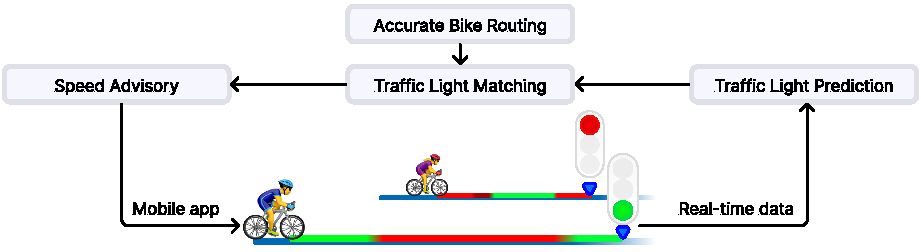
\includegraphics[width=\linewidth]{images/outline.png}
\caption{Illustration of the main components developed in this work. Each component represents one research challenge and will be solved in a separate chapter.}
\label{fig:outline}
\end{figure}

\textbf{\color{cidarkblue}Traffic Light Data for Prediction:} To provide a speed advisory for an upcoming traffic light, a prediction of the traffic light's switching behavior is required. Data from traffic lights all over the city must be collected and processed accordingly. Afterward, the collected data must be transformed into a traffic light prediction. Since a traffic light's switching behavior may depend highly on the current time and day and the detected traffic density, a reliable and accurate prediction is challenging. Furthermore, there may be data outages or errors in the streamed data, which reduce the quality and trustworthiness of the prediction. Highly accurate and trustworthy predictions are paramount for the overall effectiveness of the speed advisory.

\textbf{\color{cidarkblue}Traffic Light Matching:} The next challenge is about displaying the prediction for the correct traffic light. With many potential route choices in a vast city such as Hamburg, an automated method to match traffic lights along the way is needed. It is necessary to select a few from thousands of traffic lights, turning the traffic light matching into a search for needles in the haystack. Which traffic lights should be matched depends highly on the user's planned turns and other factors like the type of transport mode. In our case, cyclist traffic lights should be preferred. Due to the often ambiguous choice of traffic lights at an intersection, the matching algorithm has to consider multiple variants and decide on the best traffic lights. Additionally, the matching must be quick and reasonable to provide a responsive mobile application.

\textbf{\color{cidarkblue}Accurate Bike Routing:} To know which traffic lights will be along the way, this work will utilize a route-based approach. Users will select waypoints through the app, calculate a bike route based on these waypoints, and then travel along this route, as in other navigation apps. However, this also means the bike routes should follow bike paths as accurately as possible and be tailored to the user's needs, providing an accurate foundation for traffic light matching. The challenge is that existing routing foundations are designed as general-purpose maps focusing on motorists, meaning bike paths are often missing or tagged inconsistently. One key focus of this work is, thus, to find methods that allow a more accurate bike routing to enhance the overall in-app experience and provide a solid foundation for an accurate speed advisory.

\textbf{\color{cidarkblue}Speed Advisory:} The speed advisories generated by our app need to be tailored to the user's needs as well. Factors such as the road's inclination, surface quality, and bike type play a large role in selecting an optimal speed, not only when the traffic light switches to green. In some cases, users may not be able or willing to follow a speed recommendation. At the same time, potential distractions from traffic that could seriously endanger cyclists should be minimized. This brings the challenge that a good balance between displaying useful information to the user and avoiding unnecessary distractions is needed. All of these aspects need to be packaged into a mobile application, which can be distributed and directly used by people in Hamburg. Afterward, another challenge is measuring from the recorded telemetry which impacts the speed advisory had on cycling behavior. Accompanied by a user survey, the aim is to understand whether GLOSA aligns with user expectations and integrates seamlessly into their cycling routines.

Each of the presented four challenges represents one step in the ladder, which needs to be taken to ultimately judge the purposefulness of GLOSA applications in motivating more cycling.

\section{Contributions and Research Questions}



\section{How to Read This Thesis}

Each chapter in this thesis is self-contained and follows one described challenge along the processing chain of a GLOSA system. As such, each chapter can also be read separately. First, in \Cref{ch:prediction}, we will discuss the challenge of traffic light prediction, contributing to the understanding of traffic light switching patterns and real-world deployment challenges, and obtaining a functional city-scale prediction system for our bike-GLOSA app. Afterward, in \Cref{ch:matching}, we connect the traffic light prediction with the cyclist by allowing the app to match traffic lights along a preselected route. In \Cref{ch:routing}, we develop an accurate bike routing that improves traffic light matching and distance-to-signal estimation. All solutions are integrated into the final app discussed by \Cref{ch:app}, focusing on the user interface to provide the best possible speed advisory. In this chapter, we also evaluate the impact of the speed advisory on cyclist behavior. At the end of this thesis, \Cref{ch:conclusions} summarizes the gained knowledge and main results for all individual challenges and gives an overarching outlook for future studies.
